\section{Simuleringsvindauge}
\thispagestyle{fancy}

Når ein simulerer eit program kan det bli mange variablar og komponentar
å halde styr på. Derfor er det viktig å sorterer og behalde relevant informasjon, 
samt å kunne presentere den på ein god måte.

\gls{Codesys} Visualization \citep{CodesysVizualisation} er eit grafisk verktøy der ein kan presentere informasjon ved hjelp av grafiske element. 
Dette gav oss moglegheit til å presentere tankar, ventilar og pumper ved hjelp av symbol. 

Vi nytta visualiseringsverktøyet til å lage eit fullskala simuleringsvindauge, der kvar komponent vart knytt til sitt spesifikke grafiske symbol.
Vi knytta vindauget saman med programmet og kopla relevante signal.
Dette gjorde at vi hadde eit grensesnitt mot programmet og kunne enkelt simulere
forskjellige driftssituasjonar og konkludere med resultat.

Simuleringsvindauget er ikkje noko \gls{HMI} og tar ikkje omsyn til aktuelle normer og krav.

\begin{figure}[htbp]
    \centering
    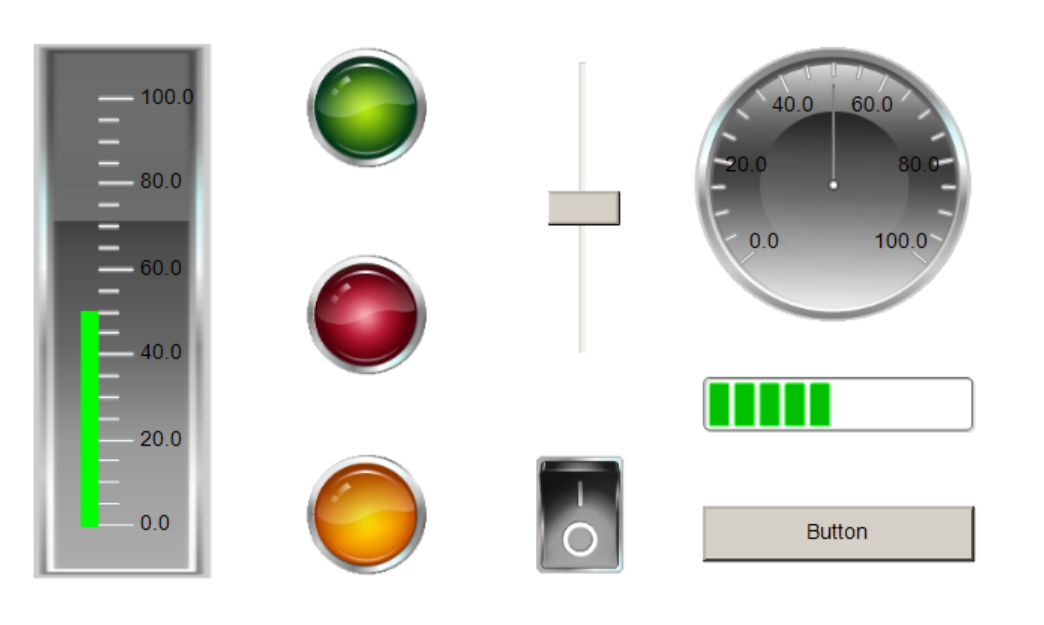
\includegraphics[width=0.8\textwidth]{Bilder/Codesys symbol.png}
    \caption{Eksempel \gls{Codesys} visualiseringselement}\label{fig:CodesysVisualisering}
\end{figure}

\newpage
